% !TeX root = ../CV note.tex
\section{Image Formation}

本讲讨论图像是如何形成的：先由最简单的针孔模型建立相机的数学描述，再引入透镜，最后讨论景深、视场、镜头像差、颜色和图像传感。

\subsection{Camera}

\subsubsection{Why Do We Need a Pinhole}

如果把数字传感器（CCD 或 CMOS）直接对着真实场景，每个传感器像素都会接收到来自场景中几乎所有点的光线，各种方向的光被平均在一起，得到的图像完全模糊。问题在于没有对光线的方向施加任何限制。

针孔相机（pinhole camera）在传感器前放置一块不透光的挡板（barrier/diaphragm），上面开一个针孔（pinhole/aperture）。绝大多数光线被挡住，只有一条光线能穿过针孔到达传感器，于是场景中的每个点只对应传感器上的一个像素，图像变得清晰。

小孔成像在中国古代已有记载。《墨经·经下》：“景到，在午有端与景长，说在端。”《经说下》：“景。光之人，煦若射，下者之人也高；高者之人也下。足蔽下光，故成景于上；首蔽上光，故成景于下。在远近有端，与于光，故景库内也。”其中已经指出倒像（“景到”）的成因是光沿直线传播并被小孔限制。

日常环境中也常出现偶然的针孔相机（accidental pinhole camera）：树叶缝隙、窗帘孔洞等会投出成像，这些成像常常不被注意或被误认为阴影。Torralba 和 Freeman 在 \textit{Accidental Pinhole and Pinspeck Cameras}（CVPR 2012）中对此做了系统研究。

\subsubsection{Mathematical Pinhole Camera Model}

物理上像平面位于针孔之后，成倒像；为了建模方便，通常把像平面平移到针孔之前，此时成的是正像，几何关系不变。设相机坐标系中物点坐标为 $(x,y,z)$，像平面上的像点坐标为 $(x',y')$，针孔到像平面的距离（焦距）为 $f$，由相似三角形得

\[
\frac{x'}{f} = \frac{x}{z}, \qquad \frac{y'}{f} = \frac{y}{z}
\]

即

\[
x' = f\frac{x}{z}, \qquad y' = f\frac{y}{z}
\]

注意这里出现了除以 $z$ 的运算，因此投影并不是线性变换，这一点后面还会展开。

\subsubsection{Coordinate Systems and Extrinsics}

成像过程涉及三个坐标系：世界坐标系（world coordinates）、相机坐标系（camera coordinates）和图像坐标系（image coordinates）。

外参（extrinsic parameters）描述如何把世界坐标中的点 $(x,y,z)$ 变换到相机坐标系，包含两部分：

\begin{itemize}
    \item 相机或物体的位置 → 平移（translation），3 个自由度
    \item 相机或物体的朝向 → 旋转（rotation），3 个自由度
\end{itemize}

合起来是刚体变换（rigid transformation），共 6 个自由度。

用齐次坐标（homogeneous coordinates）可以把平移和旋转统一写成矩阵乘法。齐次坐标把一个点表示为多一维的向量，并通过最后一维归一化：

\[
\boldsymbol{x} = (x, y, z, w) \;\cong\; \left(\frac{x}{w}, \frac{y}{w}, \frac{z}{w}, 1\right)
\]

于是平移、旋转和刚体变换分别写成

\[
T = \begin{bmatrix} I_{3\times3} & t_{3\times1} \\ 0 & 1 \end{bmatrix}, \qquad
R = \begin{bmatrix} R_{3\times3} & 0 \\ 0 & 1 \end{bmatrix}, \qquad
M = \begin{bmatrix} R_{3\times3} & t_{3\times1} \\ 0 & 1 \end{bmatrix}
\]

其中 $I$ 为单位矩阵，$t$ 为平移向量。下标只用于标注各块的形状，实际书写时可以省略。

\subsubsection{Intrinsics}

内参（intrinsic parameters）描述如何把相机坐标系中的点 $(x,y,z)$ 投影到图像平面，本质上是图像平面内的缩放加平移，用二维齐次坐标表示为

\[
\begin{bmatrix} u \\ v \\ w \end{bmatrix}
= K \begin{bmatrix} x \\ y \\ z \end{bmatrix}, \qquad
K = \begin{bmatrix}
    \alpha f & s & c_x \\
    0 & f & c_y \\
    0 & 0 & 1
\end{bmatrix}
\]

矩阵最后一行的 $[0\ 0\ 1]$ 对应透视投影（projective）；若换成 $[0\ 0\ 0\ 1]$，得到的是正交投影（orthographic）。$K$ 中各参数的含义是：

\begin{itemize}
    \item $f$：焦距
    \item $\alpha$：纵横比（aspect ratio），像素为正方形时等于 1
    \item $s$：倾斜（skew），只有当像素是平行四边形时才非零
    \item $(c_x, c_y)$：主点（principal point），当光轴与图像中心相交时等于 $(w/2, h/2)$
\end{itemize}

\subsubsection{Summary of Camera Parameters}

外参（旋转 $R$ 与平移 $t$）和内参 $K$ 合起来给出 $3\times4$ 的投影矩阵：

\[
P = K \begin{bmatrix} R_{3\times3} & t_{3\times1} \end{bmatrix}
\]

它把世界坐标中的三维点直接映射为图像平面上的二维点。

\subsubsection{Properties of Projection}

投影不是线性变换（因为要除以 $z$），但仍保留若干结构性质：

\begin{itemize}
    \item 点投影为点，直线投影为直线
    \item 角度不被保持
    \item 每一组平行线交于同一个点，称为灭点（vanishing point）
\end{itemize}

以“直线投影为直线”为例，设三维直线由一点 $\boldsymbol{X}_0 = (X_0,Y_0,Z_0,1)^T$ 和方向向量 $\boldsymbol{D} = (D_1,D_2,D_3)^T$ 参数化：

\[
\boldsymbol{X}_t = \begin{bmatrix} X_0 + tD_1 \\ Y_0 + tD_2 \\ Z_0 + tD_3 \\ 1 \end{bmatrix}
\;\cong\; \begin{bmatrix} X_0/t + D_1 \\ Y_0/t + D_2 \\ Z_0/t + D_3 \\ 1/t \end{bmatrix}
\;\xrightarrow{\;t\to\infty\;}\; \begin{bmatrix} D_1 \\ D_2 \\ D_3 \\ 0 \end{bmatrix} = \boldsymbol{X}_\infty
\]

把直线的参数方程代入投影矩阵并消去参数 $t$，得到的是图像平面上的一条直线。

$\boldsymbol{X}_\infty$ 称为无穷远点（point at infinity），它的投影就是灭点：

\[
\boldsymbol{v} \cong P\boldsymbol{X}_\infty
\]

所有方向相同的直线共享同一个灭点。当灭点位于无穷远时，对应的一组直线在图像中仍然平行。相机相对于场景的朝向决定了有几个方向的平行线在图像中汇聚，这也就是一点透视（one point perspective）、两点透视（two point perspective）和三点透视的区别。

\subsection{Lens}

\subsubsection{The Pinhole Dilemma}

\begin{itemize}
    \item 针孔太小：进入的光很少，图像很暗，需要很长的曝光时间；同时衍射（diffraction）开始起作用，同样会使图像模糊。
    \item 针孔太大：进光量增加，图像变亮，但每个像素会平均来自多个方向的光线，图像失去锐度。
\end{itemize}

因此针孔相机的成像总是偏暗而且偏慢：对于场景中的某个点，单位时间内只有极少数光线能够到达像平面，而针孔的大小又必须很小才能保证清晰。

\subsubsection{Gaussian Lens Formula}

透镜的作用是在尽可能保持理想针孔相机抽象的同时捕获更多的光，也就是允许使用大孔径并且仍然得到清晰的图像。

把针孔换成透镜后，设物距为 $z$、像距为 $z'$、焦距为 $f$。由相似三角形 $x/z = x'/z'$ 得 $x/x' = z/z'$，再结合 $(x'+x)/f = x'/z$，有

\[
\frac{1}{f} = \frac{x'+x}{x'z} = \frac{1}{z} + \frac{x}{x'z} = \frac{1}{z} + \frac{1}{z'}
\]

即高斯透镜公式（Gaussian lens equation）：

\[
\frac{1}{f} = \frac{1}{z} + \frac{1}{z'}
\]

当物体位于无穷远（$z = \infty$）时，$z' = f$，即像距等于焦距，这就是对无穷远对焦的情形。（在实际情况中，由于真实相机的焦距通常非常小
对于远处的物体和风景可以将物距当作无穷远进行考虑）

\subsection{Depth of Field}

在焦距和像平面固定之后，只有一个特定距离上的物体是“对焦”的，其他距离的点会投影成图像平面上的一个弥散圆（circle of confusion）。

% 几何：f=3，像平面在 x=6。物点 2 在 z=6（合焦，z'=6）；
% 物点 1 在 z=8（远景，z'=4.8，光线在平面之前就会聚，故摊开）；
% 物点 3 在 z=5（近景，z'=7.5，光线在平面处尚未会聚）。
\begin{center}
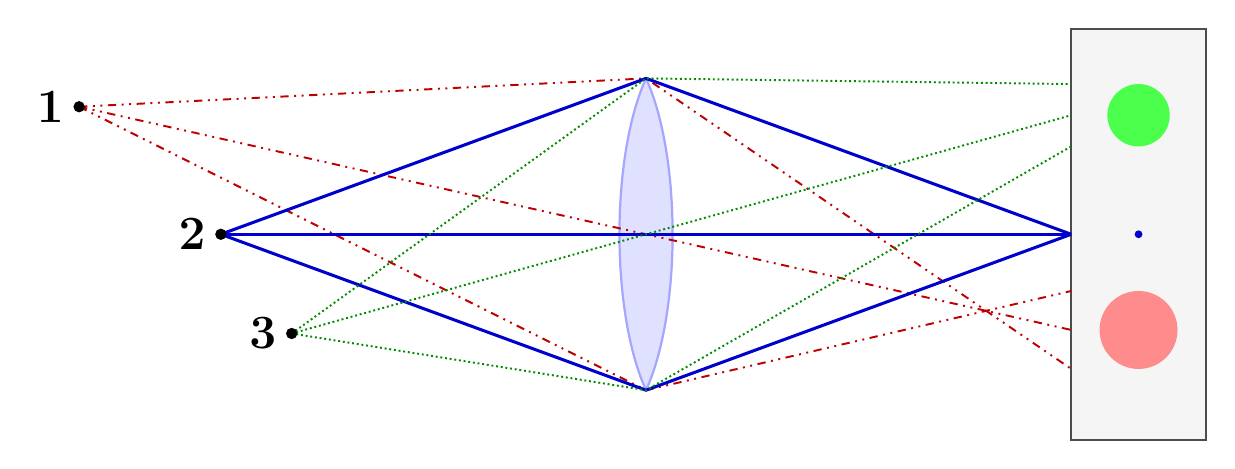
\begin{tikzpicture}[scale=0.9]
  % 像平面（右侧屏幕）
  \fill[gray!8] (6,-2.9) rectangle (7.9,2.9);
  \draw[black!70, line width=0.8pt] (6,-2.9) rectangle (7.9,2.9);

  % 双凸透镜
  \fill[blue!12]
      (0,2.2) .. controls (0.5,1.1) and (0.5,-1.1) .. (0,-2.2)
              .. controls (-0.5,-1.1) and (-0.5,1.1) .. (0,2.2);
  \draw[blue!35, line width=0.8pt]
      (0,2.2) .. controls (0.5,1.1) and (0.5,-1.1) .. (0,-2.2);
  \draw[blue!35, line width=0.8pt]
      (0,2.2) .. controls (-0.5,1.1) and (-0.5,-1.1) .. (0,-2.2);

  % 物点 1（远景，失焦）：暗红，点划线
  \draw[red!75!black, line width=0.7pt, dash dot dot] (-8,1.8) -- (0,2.2) -- (6,-1.9);
  \draw[red!75!black, line width=0.7pt, dash dot dot] (-8,1.8) -- (6,-1.35);
  \draw[red!75!black, line width=0.7pt, dash dot dot] (-8,1.8) -- (0,-2.2) -- (6,-0.8);

  % 物点 2（合焦）：蓝，实线，三条光线交于像平面上一点
  \draw[blue!80!black, line width=1.1pt] (-6,0) -- (0,2.2) -- (6,0);
  \draw[blue!80!black, line width=1.1pt] (-6,0) -- (6,0);
  \draw[blue!80!black, line width=1.1pt] (-6,0) -- (0,-2.2) -- (6,0);

  % 物点 3（近景，失焦）：绿，点线
  \draw[green!55!black, line width=0.7pt, densely dotted] (-5,-1.4) -- (0,2.2) -- (6,2.12);
  \draw[green!55!black, line width=0.7pt, densely dotted] (-5,-1.4) -- (6,1.68);
  \draw[green!55!black, line width=0.7pt, densely dotted] (-5,-1.4) -- (0,-2.2) -- (6,1.24);

  % 物点与标号
  \fill (-8,1.8) circle (0.08);
  \fill (-6,0) circle (0.08);
  \fill (-5,-1.4) circle (0.08);
  \node[left=2pt, font=\LARGE\bfseries] at (-8,1.8) {1};
  \node[left=2pt, font=\LARGE\bfseries] at (-6,0) {2};
  \node[left=2pt, font=\LARGE\bfseries] at (-5,-1.4) {3};

  % 像平面上的结果：中间合焦成点，上下两个是弥散圆
  \fill[green!70] (6.95,1.68) circle (0.44);
  \fill[blue!80!black] (6.95,0) circle (0.055);
  \fill[red!45] (6.95,-1.35) circle (0.55);
\end{tikzpicture}
\end{center}

景深（depth of field, DOF）定义为场景中看起来足够清晰（acceptably sharp）的最近物体与最远物体之间的距离。

控制景深的主要手段是光圈（aperture）大小：

\begin{itemize}
    \item 光圈越小，景深越大
    \item 但小光圈减少进光量，需要增加曝光时间，图像噪声更大
\end{itemize}

实际拍摄中的取舍是：大光圈适合拍摄孤立主体，例如夜景或人像；小光圈提供更大的景深，适合风景、流水等题材。

\subsection{Field of View}

视场（field of view, FoV）是相机所观测到的世界的角度范围。设传感器尺寸为 $d$，像距为 $z'$，视场角为 $\alpha$，则

\[
\tan\frac{\alpha}{2} = \frac{d/2}{z'}
\]

其中 $z' = (1+m)F$，$m$ 为放大率；对无穷远对焦时 $z' = F$。焦距越短，视场越大（广角）；焦距越长，视场越小（长焦）。
感受整体的风景效果，应当采用短焦镜头增大视角。拍摄远处的东西，采用长焦镜头。

\subsection{Lens Aberrations}

\subsubsection{Radial Distortion}

径向畸变（radial distortion）由透镜不完美引起，在广角镜头中尤其明显，越靠近图像边缘越显著，表现为图像内容被压缩。
负径向畸变指的是图像背离径向方向发生变形，这由于使用了超广角镜头，导致图片呈现木桶式的向外膨胀现象；正径向畸变反之，是向内陷入的现象。

建模时不再直接使用标准投影矩阵，而是分三步进行：

\begin{enumerate}
    \item 投影到“归一化”图像坐标（normalized image coordinates）：$x_n = x/z$，$y_n = y/z$
    \item 施加径向畸变：
    \[
    x_d = x_n\left(1 + k_1 r^2 + k_2 r^4\right), \qquad
    y_d = y_n\left(1 + k_1 r^2 + k_2 r^4\right)
    \]
    其中 $r^2 = x_n^2 + y_n^2$，$k_1, k_2$ 为畸变系数
    \item 施加焦距并平移到图像中心：$u = f x_d + c_x$，$v = f y_d + c_y$
\end{enumerate}

OpenCV 提供了标定和去畸变的实现。畸变对不同题材的影响不同：广角适合强调透视，标准镜头接近人眼观感，长焦则压缩空间。

\subsubsection{Chromatic Aberration}

玻璃的折射率随波长略有变化，因此简单透镜存在色差（chromatic aberration）：不同颜色的光聚焦在略微不同的距离上，表现为模糊和颜色偏移。为了减弱色差和其他像差，多数摄影镜头采用由不同玻璃元件（以及不同镀膜）组成的复合透镜（compound lens）。

\subsubsection{Vignetting}

湮灭，也叫暗角（vignetting），指亮度向图像边缘衰减的趋势。机械暗角（mechanical vignetting）是指光束的边缘部分被遮挡，从未到达像平面。这可能是由于使用两个透镜或者多个透镜的时候，光线通过了第一个透镜受到折射，没有通过第二个透镜从而导致边缘发生衰减。

\subsection{Colors}

\subsubsection{The Human Eye}

人眼与相机在结构上类似：虹膜（iris）相当于光圈，通过改变晶状体的形状对焦，视网膜（retina）相当于胶片或数字传感器。瞳孔（pupil）对应针孔或光圈，视网膜对应感光面。当眼睛正确对焦时，来自眼外物体的光被成像在视网膜上。

视网膜上有两种感光细胞：

\begin{itemize}
    \item \textbf{视杆细胞（rods）：}约 7500 万到 1.5 亿个，不参与颜色视觉，只提供灰度信息；灵敏度高，可以在夜间工作。
    \item \textbf{视锥细胞（cones）：}约 600 万到 700 万个，负责颜色视觉，在中等和高亮度条件下工作。视锥细胞有三种，光谱灵敏度峰值分别位于短波（S，420--440 nm）、中波（M，530--540 nm）和长波（L，560--580 nm）。
\end{itemize}

\subsubsection{CIE RGB}

由于人眼只有三种视锥细胞，原则上三个参数就足以描述任何一种人类颜色感觉。反过来，所有单色光（单一波长）都可以用三种适当选择的原色混合得到，即红（700.0 nm）、绿（546.1 nm）和蓝（435.8 nm）。

\subsection{Image Sensing}

\subsubsection{Imaging Pipeline}

从光到数字图像通常经过三个阶段：

\begin{enumerate}
    \item 相机镜头和机身中的物理光传输（physical light transport）
    \item 传感器芯片上的光子测量与转换（photon measurement and conversion）
    \item 图像信号处理（image signal processing, ISP）与图像压缩
\end{enumerate}

\begin{center}
\resizebox{\textwidth}{!}{%
\begin{tikzpicture}[
    font=\small,
    blk/.style={draw, fill=white, minimum height=1.15cm, text width=2.8cm,
                align=center, inner sep=2pt},
    grp/.style={draw, dashed, line width=0.7pt,
                fill={rgb,255:red,200;green,228;blue,246}},
    fl/.style={->, >=latex, line width=0.8pt},
    ln/.style={line width=0.8pt},
    cyl/.style={line width=0.8pt}
]

  % ================= 第一级：相机机身 =================
  \draw[grp] (0,1.1) rectangle (10.6,-2.3);
  \node[blk] (optics)   at (1.7,-0.35) {光学系统\\（Optics）};
  \node[blk] (aperture) at (5.1,-0.35) {光圈\\（Aperture）};
  \node[blk] (shutter)  at (8.5,-0.35) {快门\\（Shutter）};
  \draw[fl] (optics.east)   -- (aperture.west);
  \draw[fl] (aperture.east) -- (shutter.west);
  \node at (5.3,-1.85) {相机机身（Camera Body）};
  \node[align=center] at (-2.5,-0.35) {Scene\\Radiance};

  % ================= 第二级：传感器芯片 =================
  \draw[grp] (0,-3.0) rectangle (10.6,-6.4);
  \node[blk] (sensor) at (1.7,-4.5) {传感器\\（Sensor, CCD/CMOS）};
  \node[blk] (gain)   at (5.1,-4.5) {增益\\（Gain, ISO）};
  \node[blk] (adc)    at (8.5,-4.5) {模数转换\\（ADC）};
  \draw[fl] (sensor.east) -- (gain.west);
  \draw[fl] (gain.east)   -- (adc.west);
  \node at (5.3,-5.95) {传感器芯片（Sensor chip）};

  % ================= 第三级：图像信号处理器 =================
  \draw[grp] (0,-7.1) rectangle (10.6,-12.1);
  \node[blk] (demosaic) at (3.6,-8.1)  {去马赛克\\（Demosaic）};
  \node[blk] (denoise)  at (7.0,-8.1)  {去噪与锐化\\（Denoise and sharpen）};
  \draw[fl] (demosaic.east) -- (denoise.west);
  \node[blk] (wb)       at (1.7,-10.5) {白平衡\\（White Balance）};
  \node[blk] (gamma)    at (5.1,-10.5) {Gamma/曲线\\（Gamma/curve）};
  \node[blk] (compress) at (8.5,-10.5) {压缩\\（Compress）};
  \draw[fl] (wb.east)    -- (gamma.west);
  \draw[fl] (gamma.east) -- (compress.west);
  \node at (5.3,-11.65) {图像信号处理器（ISP）};

  % ================= 级间连线 =================
  % 相机机身 → 传感器芯片
  \draw[fl] (shutter.east) -- (11.8,-0.35) -- (11.8,-2.7) -- (-1.3,-2.7)
            -- (-1.3,-4.5) -- (sensor.west);

  % 传感器芯片 → RAW
  \draw[fl] (adc.east) -- (13.2,-4.5);

  % 传感器芯片 → 图像信号处理器
  \draw[fl] (11.8,-4.5) -- (11.8,-6.8) -- (-1.3,-6.8) -- (-1.3,-8.1)
            -- (demosaic.west);

  % 去噪与锐化 → 白平衡（ISP 内部回绕，绕行线在虚线框内）
  \draw[fl] (denoise.east) -- (10.0,-8.1) -- (10.0,-9.5) -- (0.6,-9.5)
            -- (0.6,-10.5) -- (wb.west);

  % 图像信号处理器 → JPEG
  \draw[fl] (compress.east) -- (13.2,-10.5);

  % ================= 输出：RAW / JPEG =================
  % RAW 数据库
  \fill[gray!25] (13.2,-3.7) -- (13.2,-5.3)
      arc[start angle=180, end angle=360, x radius=1.2, y radius=0.3]
      -- (15.6,-3.7) -- cycle;
  \draw[cyl] (13.2,-3.7) -- (13.2,-5.3)
      arc[start angle=180, end angle=360, x radius=1.2, y radius=0.3]
      -- (15.6,-3.7);
  \draw[cyl, fill=gray!45] (14.4,-3.7) ellipse (1.2 and 0.3);
  \node at (12.55,-4.2) {RAW};

  % JPEG 数据库
  \fill[gray!25] (13.2,-9.7) -- (13.2,-11.3)
      arc[start angle=180, end angle=360, x radius=1.2, y radius=0.3]
      -- (15.6,-9.7) -- cycle;
  \draw[cyl] (13.2,-9.7) -- (13.2,-11.3)
      arc[start angle=180, end angle=360, x radius=1.2, y radius=0.3]
      -- (15.6,-9.7);
  \draw[cyl, fill=gray!45] (14.4,-9.7) ellipse (1.2 and 0.3);
  \node at (12.55,-10.2) {JPEG};

\end{tikzpicture}%
}
\end{center}

\subsubsection{Shutter}

焦平面快门（focal plane shutter）位于图像传感器或胶片的正前方。多数数码相机使用机械快门与电子快门的组合。快门速度（即曝光时间）决定到达传感器的光量，进而决定图像是过曝、欠曝、模糊还是含噪。

\subsubsection{Sensor}

\begin{itemize}
    \item \textbf{CCD}：电荷在像素之间逐个移动，最终在输出节点统一转换为电压。
    \item \textbf{CMOS}：在每个像素内部完成电荷到电压的转换，目前是标准方案。
\end{itemize}

\subsubsection{Color Filter Array and Demosaicing}

为了测量颜色，像素按特定阵列排布，最常见的是 Bayer RGB 图案：每个 $2\times2$ 子块包含 2 个绿色、1 个蓝色和 1 个红色滤镜，每个滤镜覆盖一个像素传感器。这样每个像素只能测到一个通道，缺失的其他通道由邻域插值估计，这个过程称为去马赛克（demosaicing）。
一般的方法是在图像上进行双线性插值。

绿色滤镜占总数的一半，是因为人眼的亮度敏感函数（luminance sensitivity function）在绿色波段响应最强。

\subsubsection{Gamma Correction}

人眼对暗部区域的强度差异更加敏感，因此在离散化之前对强度或颜色做非线性变换是有利的，在读取时再撤销这一变换。通常取

\[
Y' = Y^{1/\gamma}
\]
这样可以给暗部留下更大的区间，最后离散化的时候梯度会更加细密，能够反映出更多细节，简而言之就是能用有限的空间牺牲一点“亮”和“很亮”的区别，保存“黑”和“灰的区别”。
同时早期的硬件输出的时候是非线性的，可以抵消一部分硬件问题。在当代，Gamma校正主要用于图像增强和特征值提取算法。

\subsection{Summary}

\begin{itemize}
    \item \textbf{相机：}针孔模型；世界坐标、相机坐标与图像坐标之间的变换；内参与外参；$3\times4$ 投影矩阵。
    \item \textbf{透镜：}透镜允许大孔径同时保持图像清晰；高斯透镜公式 $\frac{1}{f} = \frac{1}{z} + \frac{1}{z'}$。
    \item \textbf{景深：}由光圈控制，小光圈景深大但进光少、噪声大。
    \item \textbf{视场：}由传感器尺寸和像距决定，焦距越短视场越大。
    \item \textbf{畸变：}径向畸变、色差、暗角。
    \item \textbf{颜色与传感：}视杆与视锥细胞、CIE RGB、Bayer 阵列与去马赛克、Gamma 校正。
\end{itemize}

